\documentclass{article}
\usepackage{tikz}
\begin{document}
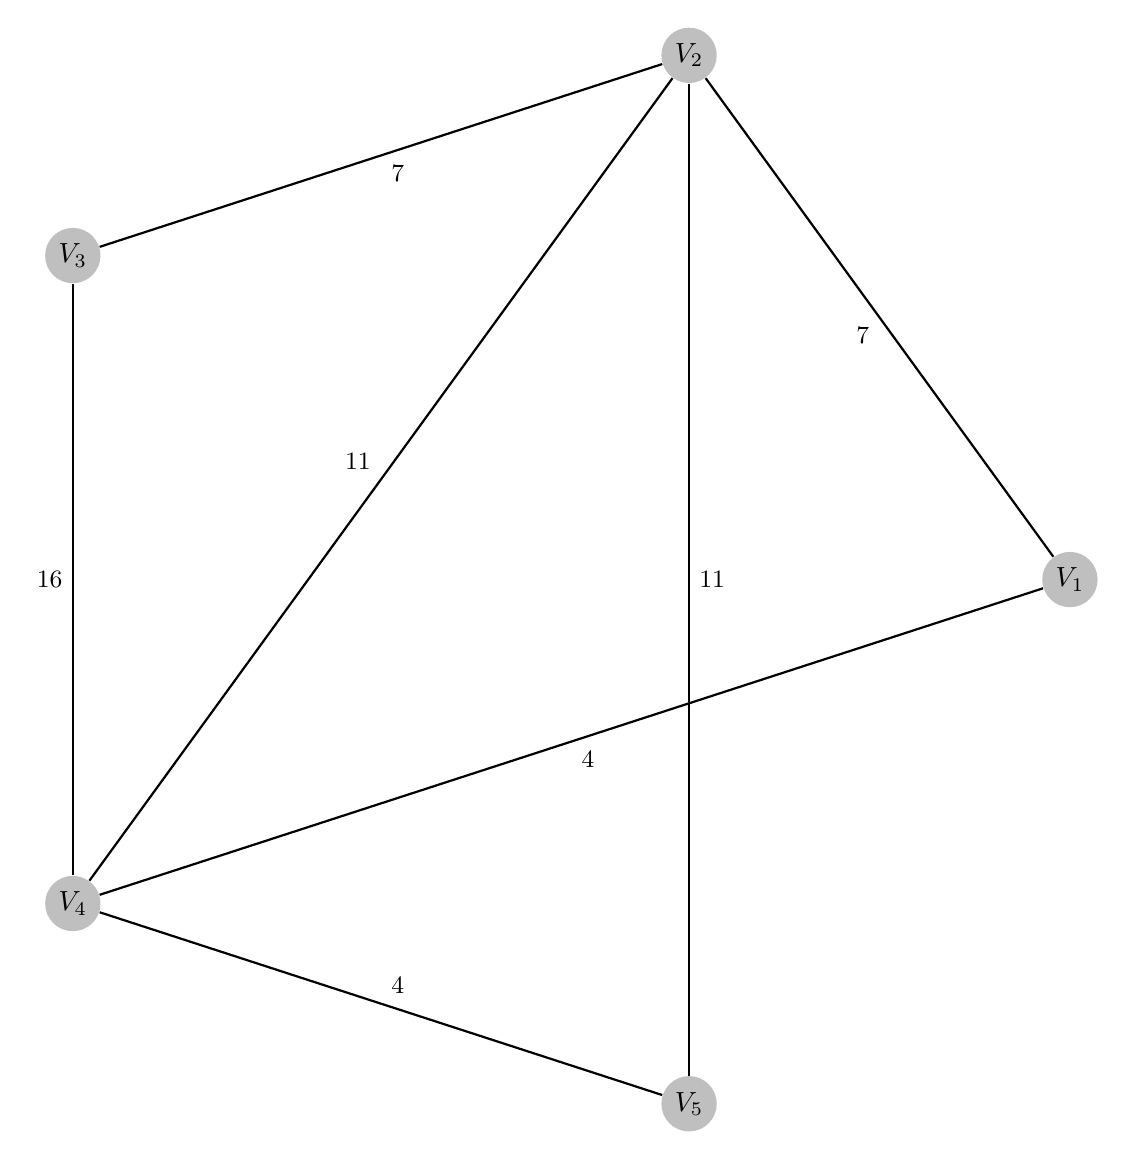
\begin{tikzpicture}[auto]
\tikzstyle{vertex}=[circle,fill=black!25,minimum size=20pt,inner sep=0pt]
\tikzstyle{edge} = [draw,thick,-]
\tikzstyle{weight} = [font=\small]
\def \radius {7cm}
\node[vertex] (1) at ({360/5 * (0 )}:\radius) {$V_{1}$};
\node[vertex] (2) at ({360/5 * (1 )}:\radius) {$V_{2}$};
\node[vertex] (3) at ({360/5 * (2 )}:\radius) {$V_{3}$};
\node[vertex] (4) at ({360/5 * (3 )}:\radius) {$V_{4}$};
\node[vertex] (5) at ({360/5 * (4 )}:\radius) {$V_{5}$};
\path[edge] (1) -- node[weight] {$7$} (2);
\path[edge] (1) -- node[weight] {$4$} (4);
\path[edge] (2) -- node[weight] {$11$} (5);
\path[edge] (2) -- node[weight] {$7$} (3);
\path[edge] (4) -- node[weight] {$16$} (3);
\path[edge] (4) -- node[weight] {$11$} (2);
\path[edge] (4) -- node[weight] {$4$} (5);
\end{tikzpicture}
\end{document}
